\documentclass[11pt,a4paper]{article}
\usepackage[margin=1in]{geometry}
\usepackage[T1]{fontenc}
\usepackage{lmodern}
\usepackage{microtype}
\usepackage{amsmath}
\usepackage{xcolor}
\definecolor{kthblue}{HTML}{004791}
\usepackage[hyphens,spaces,obeyspaces]{xurl}
\usepackage{booktabs}
\usepackage{tabularx}
\usepackage{array}
\usepackage{needspace}
\usepackage{float}
\usepackage{enumitem}
\usepackage{graphicx}
\usepackage{fancyhdr}
\usepackage{parskip}
\usepackage{hyperref}

\newcolumntype{Y}{>{\raggedright\arraybackslash}X}
\emergencystretch=2em
\setlength{\tabcolsep}{5pt}
\renewcommand{\arraystretch}{1.18}
\renewcommand{\contentsname}{}
\newcommand{\tocentry}[1]{\addcontentsline{toc}{section}{#1}}

\hypersetup{
    colorlinks=true,
    linkcolor=kthblue,
    urlcolor=kthblue,
    pdftitle={Applied GPU Programming -- Assignment 2},
    pdfauthor={Group 40: Yuanyu Zhang, Hongen Wang, Xinyang Li},
}
\title{Applied GPU Programming -- Assignment 2}
\author{Group 40 -- Yuanyu Zhang, Hongen Wang, Xinyang Li}
\date{20 November 2026}

\pagestyle{fancy}
\fancyhf{}
\fancyhead[L]{\small Applied GPU Programming -- Group 40}
\fancyhead[R]{\small Assignment 2}
\fancyfoot[C]{\small \thepage}
\renewcommand{\headrulewidth}{0.4pt}
\setlength{\headheight}{14pt}

\begin{document}

\pagenumbering{gobble}
\hypersetup{pageanchor=false}
\begin{titlepage}
\thispagestyle{empty}
\centering
\vspace*{1.0cm}

\begingroup
\setlength{\fboxsep}{12pt}
\colorbox{kthblue}{
\includegraphics[height=2.8cm]{kth-logo.png}}
\endgroup

\vspace{0.35cm}
{\footnotesize KTH Electrical Engineering and Computer Science}

\vspace{1.6cm}

{\LARGE\bfseries Assignment 2\\[0.45cm]
1D Convolution, Tiled Matrix Multiplication\\[0.25cm]
and Llama~2 Inference on the GPU}

\vspace{1.2cm}

{\small Applied GPU Programming \textperiodcentered\ HT26}

\vfill

{\large Group 40}\\[0.55cm]
{\normalsize Yuanyu Zhang \textperiodcentered\ Hongen Wang \textperiodcentered\ Xinyang Li}

\vspace{1.4cm}

{\small Stockholm, 20 November 2026}
\vspace*{0.3cm}
\end{titlepage}
\hypersetup{pageanchor=true}
\pagenumbering{arabic}

\tableofcontents
\vspace{1.5em}

\section*{Experimental environments}
\tocentry{Experimental environments}
\begin{table}[H]
\centering
\begin{tabularx}{\textwidth}{@{}lYYY@{}}
\toprule
\textbf{Question} & \textbf{GPU and system} & \textbf{CUDA and profilers} & \textbf{Purpose} \\
\midrule
Q1 & RTX 3060 Laptop GPU (CC 8.6, 30 SMs), Windows 11 + WSL2 Ubuntu 24.04, driver 566.36 & CUDA 12.6.85, Nsight Systems 2026.6.1, Nsight Compute 2024.3.2 & Timing, correctness and profiling \\
Q2 & Tesla T4, Google Colab & CUDA 13.0.88, Nsight Compute & Correctness, timing and occupancy \\
Bonus & Tesla T4, Google Colab & CUDA 13.0.88 & CPU/GPU mover correctness and timing \\
Q3 & Tesla T4, Google Colab & CUDA 13.0.88, Nsight Systems 2025.3.1 & Throughput, correctness and profiling \\
\bottomrule
\end{tabularx}
\end{table}

Kernel times in Q1 are GPU-side durations from Nsight Systems, taken as the median of 102 launches. We did not use CUDA events for this. Under WSL2 the event time of 100 back-to-back launches (6--17\,\(\mu\)s per launch) mostly measures launch overhead and changes a lot from run to run.

% =====================================================================
\clearpage
\section*{Question 1 --- 1D Convolution}
\tocentry{Question 1 --- 1D Convolution}

\texttt{conv1d.cu} completes the course skeleton. We added a \texttt{width} argument to both kernels because the skeleton signatures have no length parameter. Both kernels use one thread per output element and \(\lceil N/T\rceil\) blocks of \(T=\) \texttt{TILE\_WIDTH} threads. \texttt{convolution\_1D\_basic} reads the inputs and the mask directly from global memory. In \texttt{convolution\_1D\_tiled}, each block first copies its \(T\) inputs, two halo elements on each side and the 5 mask values into shared memory, and then computes from there. Inputs outside the array count as 0. The two kernels and the CPU reference give identical outputs.

\subsection*{1. Application domains}
Image processing and computer vision use convolution for blurring and edge detection, for example with Gaussian or Sobel filters. In audio and signal processing, FIR filters and noise reduction are 1D convolutions over the samples. Convolutional neural networks are built from convolution layers.

\subsection*{2. Global-memory reads and writes}
\textbf{Basic kernel.} Every output needs 5 inputs and 5 mask values. At the two ends of the array some neighbours lie outside and are skipped (2 + 1 at the start, 1 + 2 at the end), which saves 6 input reads and 6 mask reads.

\textbf{Tiled kernel.} Every input element is read once into its own tile. Each of the \(B-1\) boundaries between neighbouring tiles adds 4 reads, since both blocks load 2 elements of the other tile as halo. Every block also reads the mask once. With \(B=\lceil N/T\rceil\):
\[
R_\text{basic}=2(5N-6)=10N-12, \qquad
R_\text{tiled}=N+4(B-1)+5B, \qquad
W_\text{basic}=W_\text{tiled}=N.
\]
Both kernels write each output once. For \(N=16{,}384\) and \(T=128\) the basic kernel reads 163,828 times and the tiled kernel 17,532 times, about 9.3 times fewer. This counts load instructions in the code. Nsight Compute reports a 74.7\% L1 hit rate for the basic kernel (3.7\% for the tiled one), so the difference in DRAM traffic is smaller than the count suggests.

\subsection*{3. Results and tile size}
\begin{figure}[H]
\centering
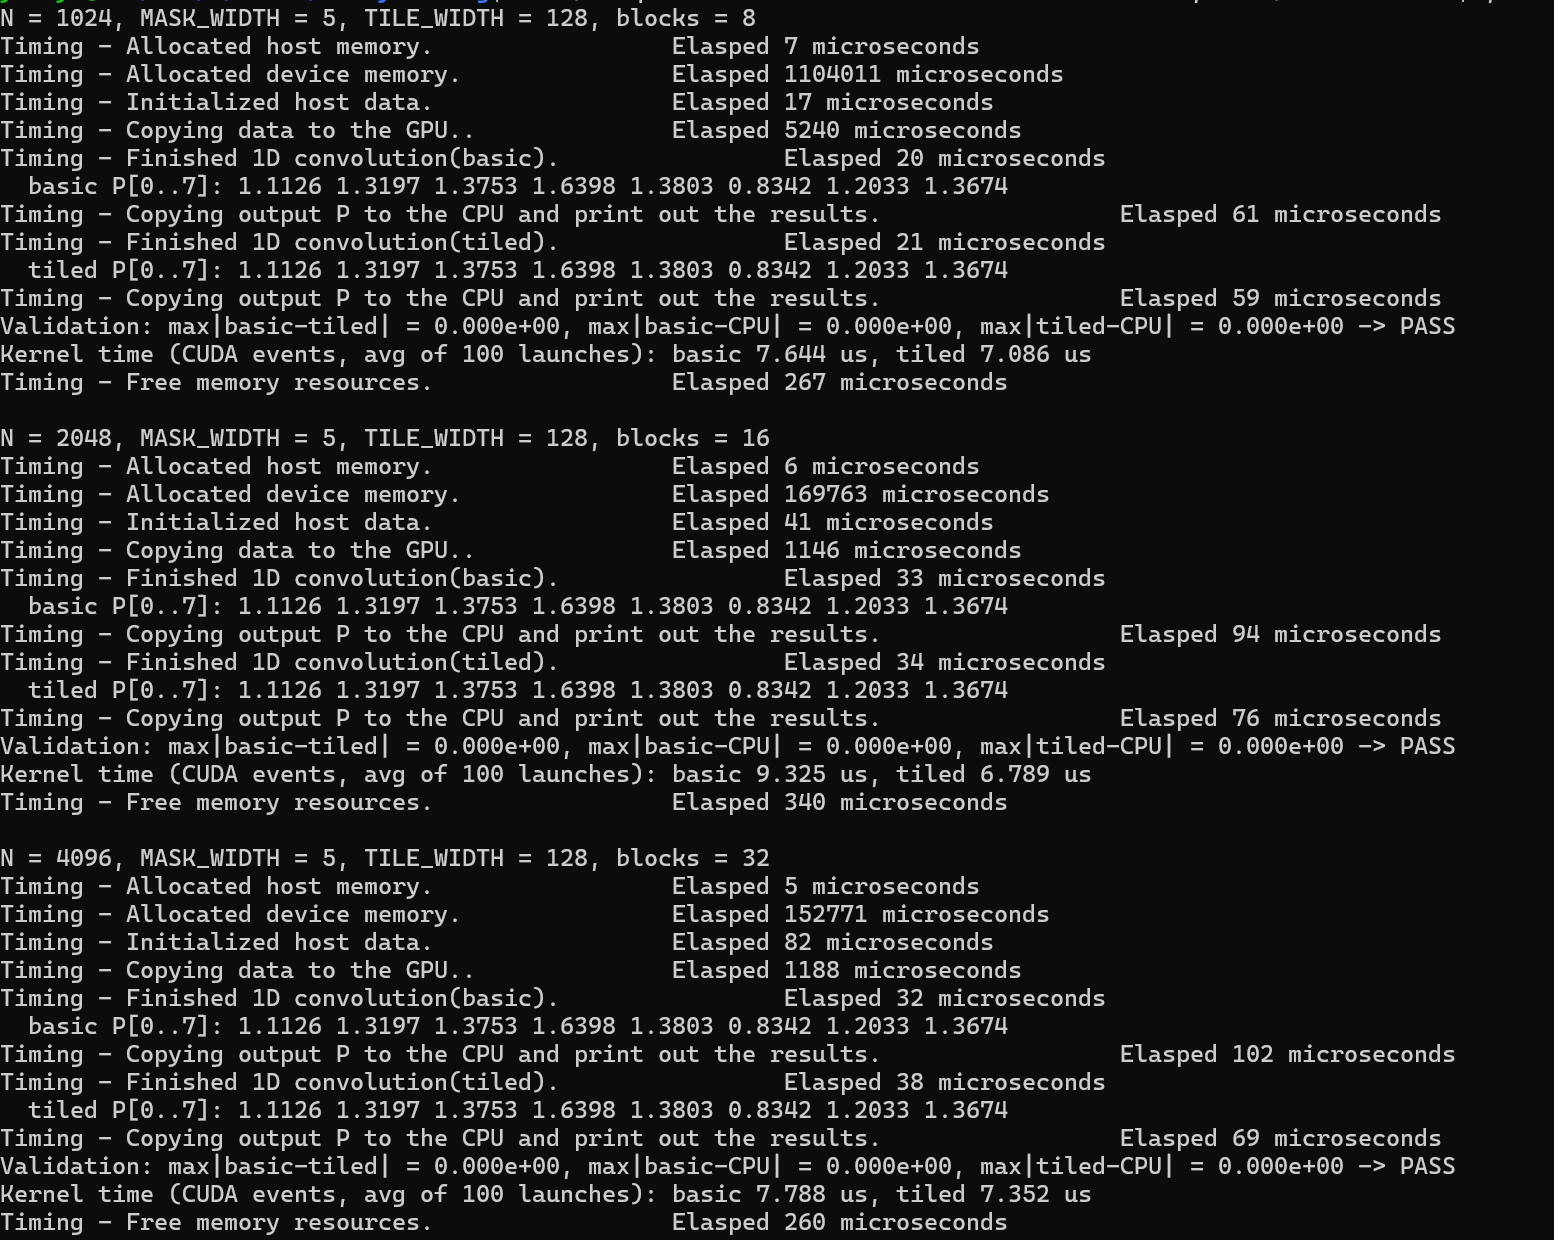
\includegraphics[width=0.73\textwidth]{Q1/results/screenshots/q13_output_1.png}\\[4pt]
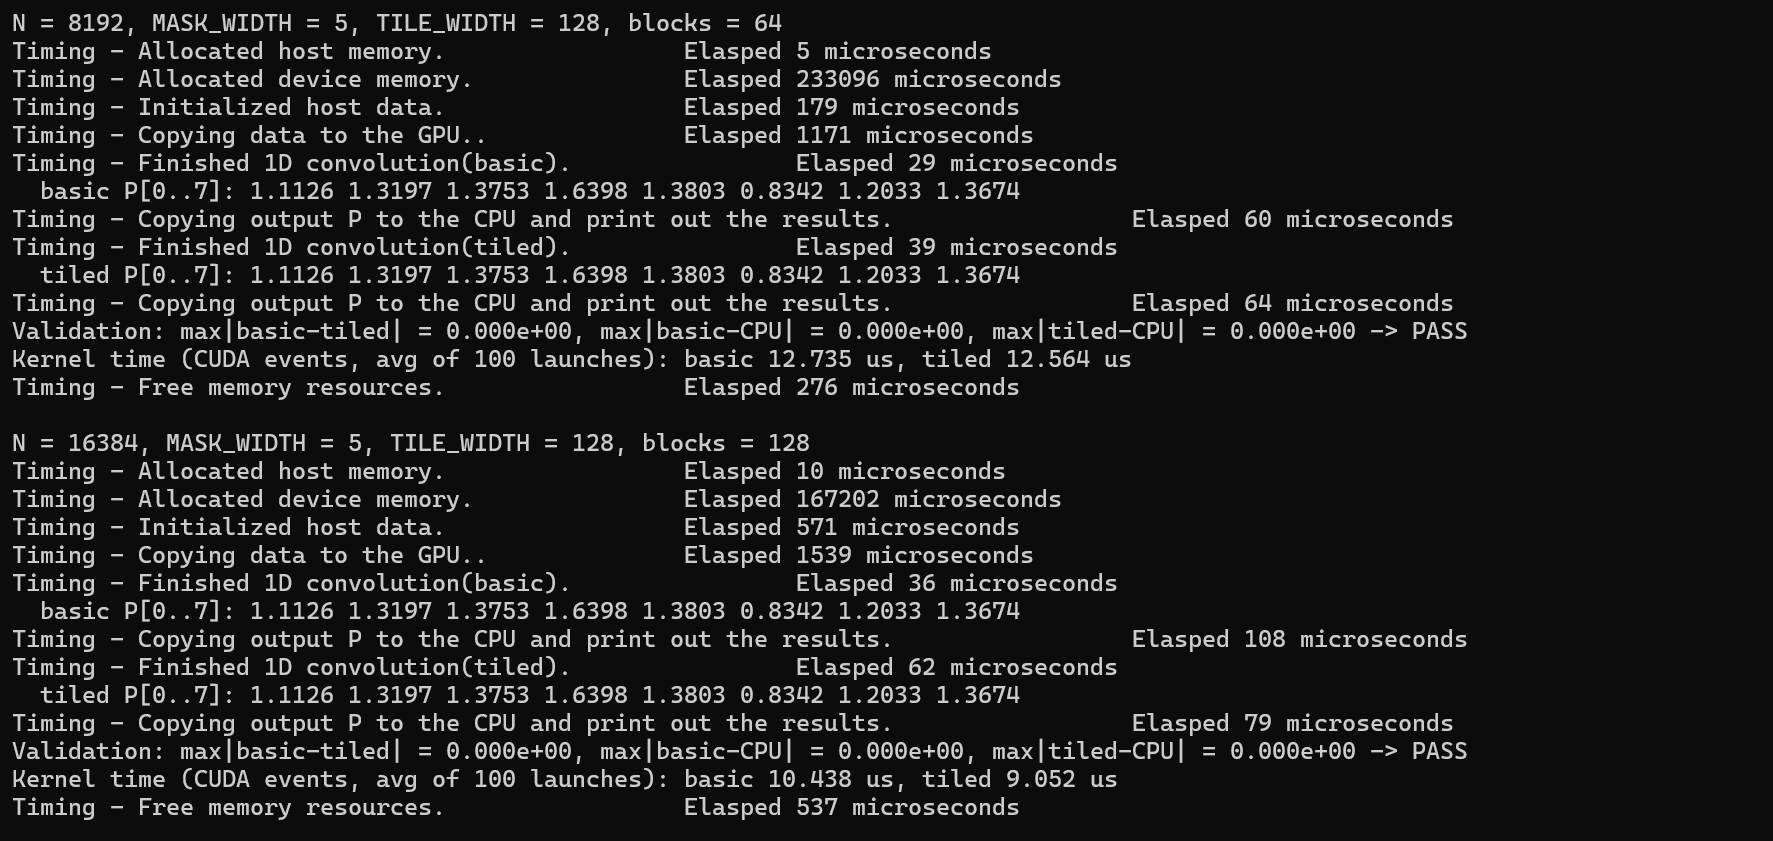
\includegraphics[width=0.73\textwidth]{Q1/results/screenshots/q13_output_2.png}
\caption{Output for \(N=1{,}024\) to \(16{,}384\) with \texttt{TILE\_WIDTH} = 128. All five runs pass the validation.}
\label{fig:q1-output}
\end{figure}

\texttt{TILE\_WIDTH} is a compile-time constant, so we compiled one binary per tile size and measured both kernels with Nsight Systems (Table~\ref{tab:q1-sweep}).

\begin{table}[H]
\centering
\begin{tabular}{@{}rrrrrrrr@{}}
\toprule
\(N\) & \(T=32\) & 64 & 128 & 256 & 512 & 1024 & Basic (\(T=128\)) \\
\midrule
1,024  & 1.73 & \textbf{1.54} & 1.57 & 1.60 & 1.73 & 1.79 & 1.22 \\
2,048  & 1.76 & \textbf{1.57} & \textbf{1.57} & 1.60 & 1.70 & 1.92 & 1.25 \\
4,096  & 1.86 & 1.66 & 1.63 & \textbf{1.60} & 1.70 & 1.89 & 1.28 \\
8,192  & 1.95 & 1.73 & \textbf{1.70} & 1.73 & 1.73 & 1.92 & 1.35 \\
16,384 & 2.82 & 1.82 & \textbf{1.79} & 1.82 & 1.89 & 1.92 & 1.50 \\
\bottomrule
\end{tabular}
\caption{Tiled kernel time in \(\mu\)s per tile size (median of 102 launches, fastest in bold) and the basic kernel for comparison.}
\label{tab:q1-sweep}
\end{table}

\(T=128\) has the lowest tiled time for \(N=2{,}048\), \(8{,}192\) and \(16{,}384\). For 1,024 and 4,096 it is 32\,ns behind the best tile. That is one step of the timer, so we use \(T=128\) for all sizes.

The reason is the per-SM limits of the GPU. It has 30 SMs, and each SM holds at most 16 blocks and 48 warps (1,536 threads). With \(T=32\) or 64, 16 blocks give only 512 or 1,024 threads per SM. Small tiles also repeat the halo and mask loads more often, and \(T=32\) is clearly the slowest at \(N=16{,}384\) (2.82\,\(\mu\)s). Large tiles give few blocks. For \(N=1{,}024\), \(T=1{,}024\) runs as a single block on one SM, and its barrier waits for 32 warps. \(T=128\) is the smallest multiple of 32 above 96 threads (\(1{,}536/16\)), so an SM can be filled, and \(N=16{,}384\) still gives 128 blocks, more than four per SM.

The tiled kernel is 0.3--0.4\,\(\mu\)s slower than the basic kernel for every \(N\). The input is at most 64\,KB and stays in the L1 and L2 caches, so the repeated loads of the basic kernel cost little. Each tiled block has extra work: the barrier, the stores to shared memory, the mask copy and the halo branches. The branches cause divergence. Nsight Compute shows 29.3 active threads per warp on average, against 32 for the basic kernel.

\subsection*{4. Profiling}
We profiled \(N=16{,}384\) with \(T=128\), which gives 128 blocks.

\begin{figure}[H]
\centering
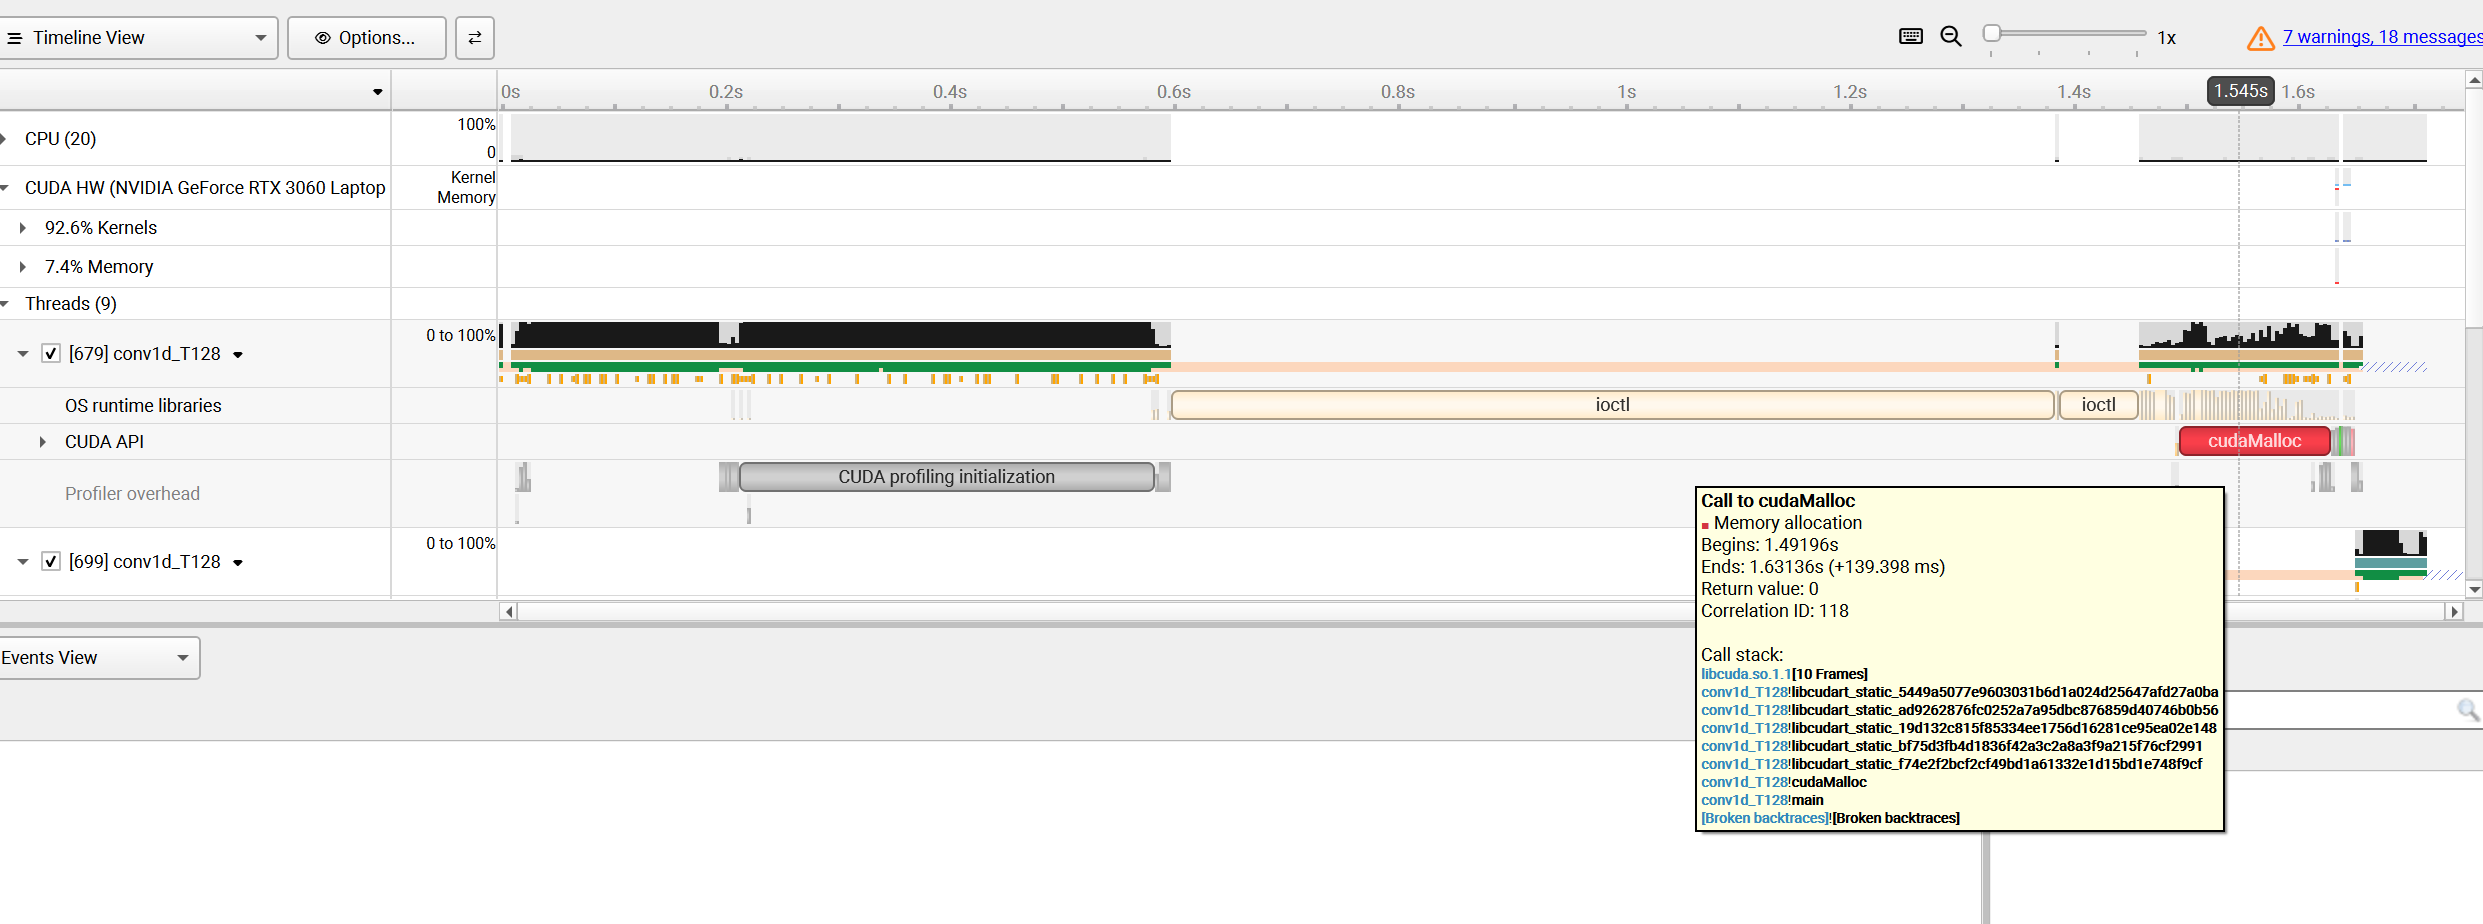
\includegraphics[width=0.85\textwidth]{Q1/results/screenshots/nsys_overview.png}
\caption{Nsight Systems timeline of the whole program. The tooltip shows the first \texttt{cudaMalloc}.}
\label{fig:q1-nsys-overview}
\end{figure}

\textbf{Hotspot.} In the whole program the first \texttt{cudaMalloc} takes 139\,ms (Figure~\ref{fig:q1-nsys-overview}), 88.8\% of the CUDA API time, because it creates the CUDA context. All kernels and memory copies together use about 0.36\,ms of GPU time.

\begin{figure}[H]
\centering
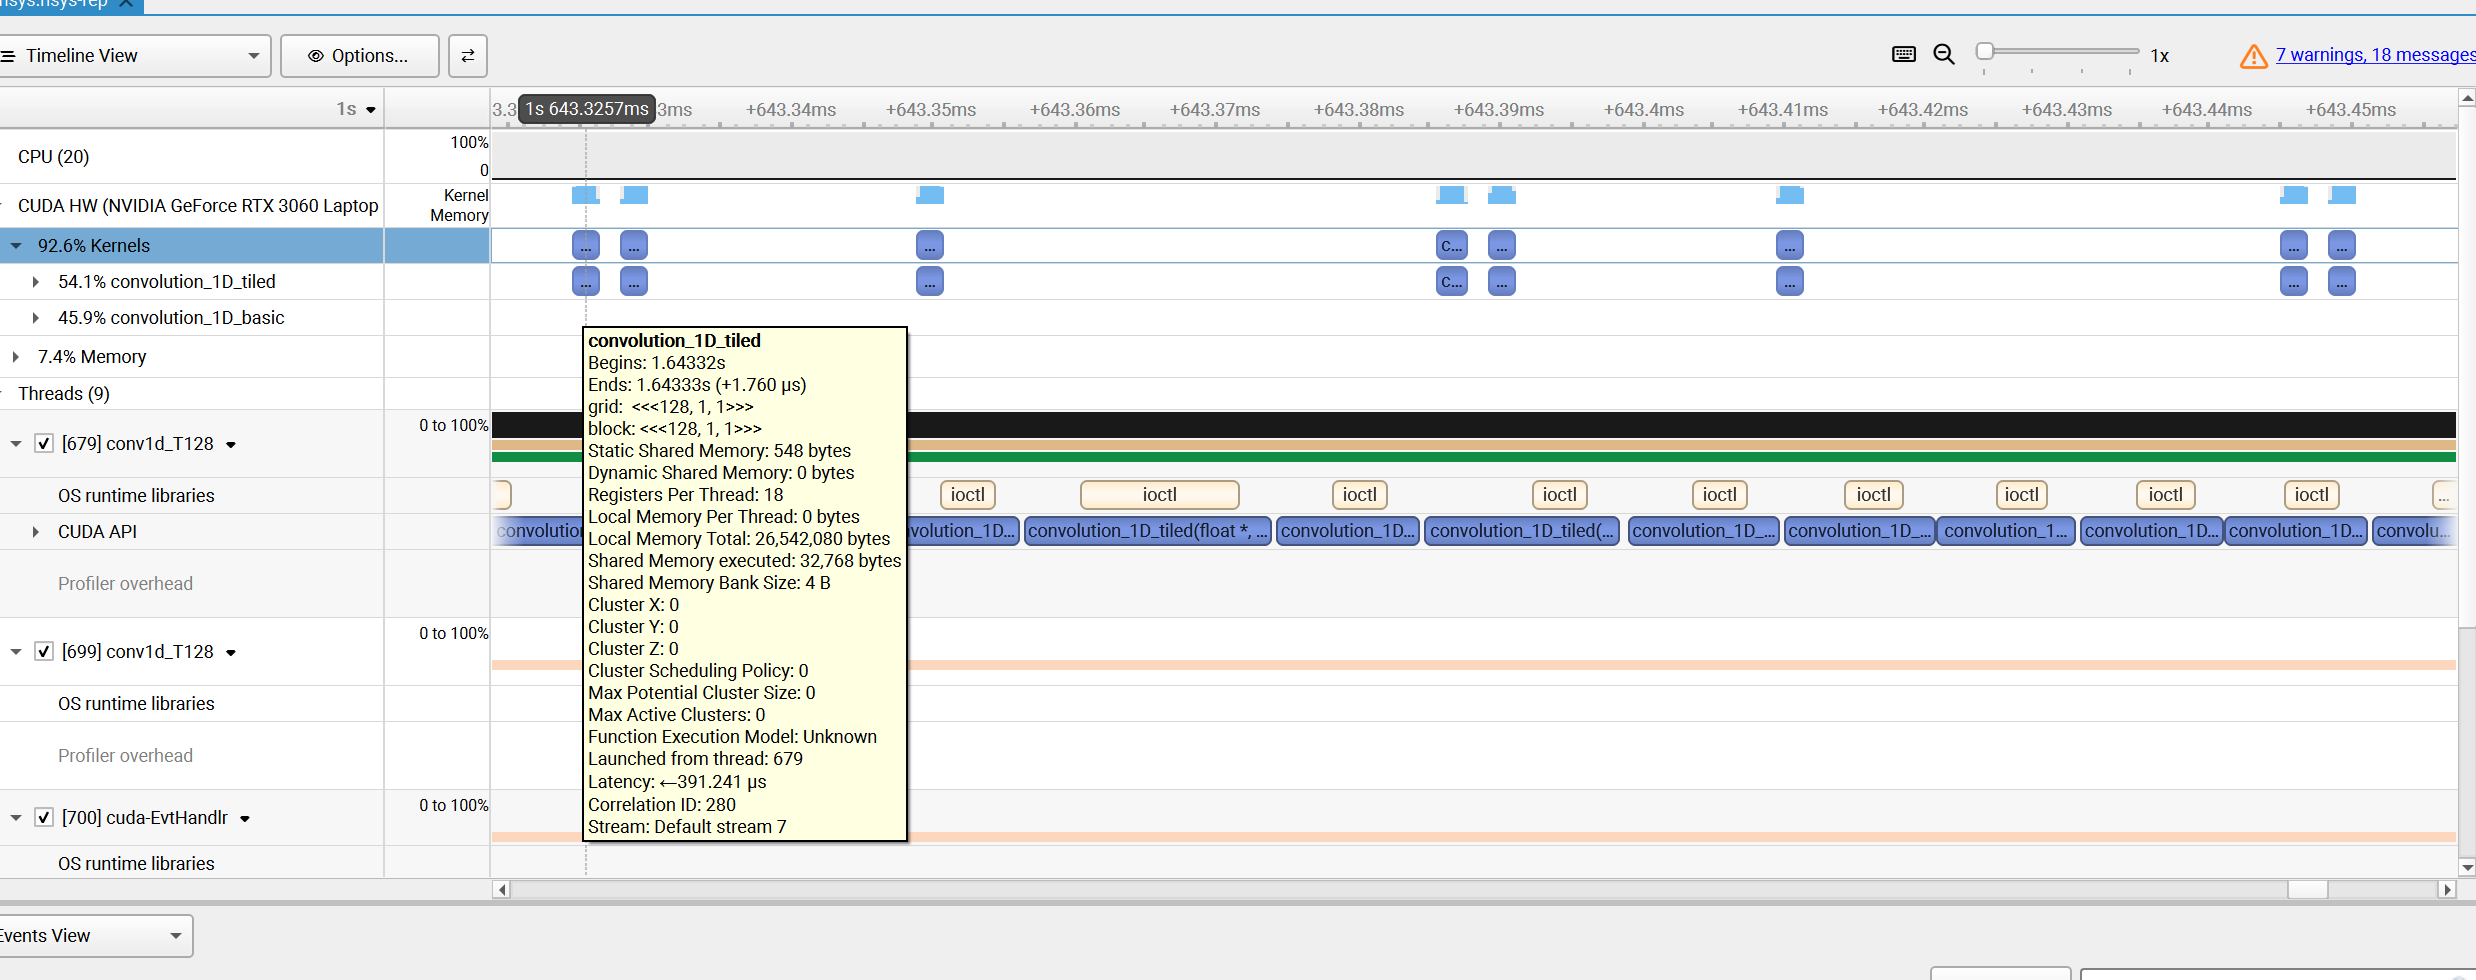
\includegraphics[width=0.85\textwidth]{Q1/results/screenshots/nsys_kernels_zoom.png}
\caption{Zoomed timeline of the kernel launches. The tooltip shows one \texttt{convolution\_1D\_tiled} launch.}
\label{fig:q1-nsys-zoom}
\end{figure}

In Figure~\ref{fig:q1-nsys-zoom}, one tiled launch runs for 1.76\,\(\mu\)s on the GPU, while the median \texttt{cudaLaunchKernel} call takes 7.6\,\(\mu\)s on the CPU. The GPU is therefore idle between kernels most of the time.

Inside the kernel, memory and compute throughput are both 11\% of peak (Table~\ref{tab:q1-ncu}). In 90\% of the cycles no warp is ready to issue. The two largest stall reasons are misses in the immediate constant cache, which holds the kernel arguments, and scoreboard waits on global loads. The kernel is limited by latency, and there are too few warps per SM to hide it.

\begin{table}[H]
\centering
\small
\begin{tabularx}{\textwidth}{@{}YrYr@{}}
\toprule
\textbf{Metric} & \textbf{Value} & \textbf{Metric} & \textbf{Value} \\
\midrule
Memory / compute throughput & 11.4\% / 11.4\% & Occupancy (theor.\ / achieved) & 100\% / 33.6\% \\
Shared memory per block & 548\,B + 1\,KB driver & Block limit: warps / shared mem & 12 / 19 \\
Shared memory configuration & 32.8\,KB & Cycles with no eligible warp & 89.8\% \\
\bottomrule
\end{tabularx}
\caption{Nsight Compute metrics of \texttt{convolution\_1D\_tiled} (\(N=16{,}384\), \(T=128\)).}
\label{tab:q1-ncu}
\end{table}

\textbf{Shared memory and occupancy.} Each block uses 548 bytes of shared memory, 528 for the tile and 20 for the mask. The driver reserves another 1\,KB per block. With about 4.3 blocks on each SM this adds up to 6.7\,KB, or 20\% of the 32.8\,KB configured. Shared memory would allow 19 blocks per SM and the warp count allows 12, so neither limits occupancy here. The achieved occupancy of 33.6\% (16.1 of 48 warps) comes from the grid size. 128 blocks of 4 warps over 30 SMs is about 17 warps per SM, and the grid fills only 0.36 of one wave.

\textbf{Shared-memory capacity.} We set the carveout with \texttt{cudaFuncSetAttribute} (Table~\ref{tab:q1-carveout}).

\begin{table}[H]
\centering
\begin{tabular}{@{}lrrrr@{}}
\toprule
\textbf{Carveout} & \textbf{Shared memory} & \textbf{Block limit} & \textbf{Occupancy} & \textbf{Duration} \\
\midrule
not set & 32.8\,KB & 19 & 100\% / 33.6\% & 3.33\,\(\mu\)s \\
0\% & 8.2\,KB & 4 & 33.3\% / 28.7\% & 4.22\,\(\mu\)s \\
25\% / 50\% / 100\% & 102.4\,KB & 61 & 100\% / 33.2--33.5\% & 3.36--3.39\,\(\mu\)s \\
\bottomrule
\end{tabular}
\caption{Effect of the carveout. Block limit from shared memory, theoretical / achieved occupancy, Nsight Compute duration.}
\label{tab:q1-carveout}
\end{table}

For 25\%, 50\% and 100\% the driver picks 102.4\,KB. Duration and occupancy stay as with the default 32.8\,KB, because shared memory was not the limit before. More capacity does not help. With 0\% only 8.2\,KB is available. Then 4 blocks of about 1.6\,KB fill an SM, theoretical occupancy drops to 33\%, and the kernel takes 4.22\,\(\mu\)s instead of 3.33\,\(\mu\)s, 27\% slower.

% =====================================================================
\clearpage
\section*{Question 2: Tiled matrix multiplication}
\tocentry{Question 2: Tiled matrix multiplication}

\texttt{Q2/gemm\_tiled.cu} extends the Assignment 1 GEMM with
\texttt{tiled\_gemm()}. The naive kernel assigns one output element to each
thread. A tiled block computes a \texttt{tileY}-by-\texttt{tileX} output tile
and stages A and B in dynamic shared memory, using reduction chunks of
\texttt{tileX}. Out-of-range elements are zero, which handles partial tiles
without a separate reduction tail. The program validates every output element
against a full CPU reference. Each GPU time is the median of 10 CUDA-event
measurements after one warm-up launch, excluding copies. All runs use float on
the Colab Tesla T4.

\subsection*{1. Global-memory reads}
For A of size \(M\times K\) and B of size \(K\times N\), each of the \(MN\)
outputs reads \(K\) elements from each input in the naive kernel:
\[
R_\text{naive}=2MNK.
\]
A tiled row block loads its A slab once for each of \(\lceil N/t_x\rceil\)
column blocks. B is loaded once for each of \(\lceil M/t_y\rceil\) row blocks:
\[
R_\text{tiled}=MK\left\lceil\frac{N}{t_x}\right\rceil
              +KN\left\lceil\frac{M}{t_y}\right\rceil
 \approx MNK\left(\frac1{t_x}+\frac1{t_y}\right).
\]
Both kernels write C once. For \(1024^3\), the naive kernel performs
2,147,483,648 operand reads. Square tiles of width 8, 16 and 32 reduce this
count to 268,435,456, 134,217,728 and 67,108,864. These counts describe loads
in the source. Repeated naive loads may hit in the cache, so the counts do not
represent DRAM transactions.

\subsection*{2. Square \(1024\times1024\) matrices}
\begin{figure}[H]
\centering
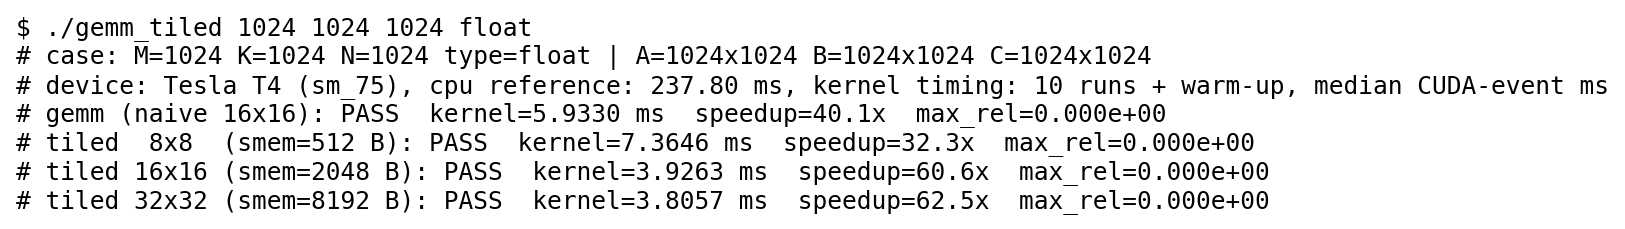
\includegraphics[width=\textwidth]{Q2/results/screenshots/q2_1024_output.png}
\caption{Output for the square case. Every kernel passes full validation.}
\label{fig:q2-square}
\end{figure}

The 16 tile takes 3.9263\,ms, 1.51 times as fast as naive GEMM
(5.9330\,ms). Increasing the tile to 32 reduces the time to 3.8057\,ms, a
\(1.56\times\) speed-up. The 8 tile is slower than naive at 7.3646\,ms because its
smaller reduction in global loads, larger grid and synchronization overhead
outweigh the tiling benefit. The CPU reference takes 237.80\,ms.

\subsection*{3. Non-divisible \(513\times8192\times1023\) case}
\begin{figure}[H]
\centering
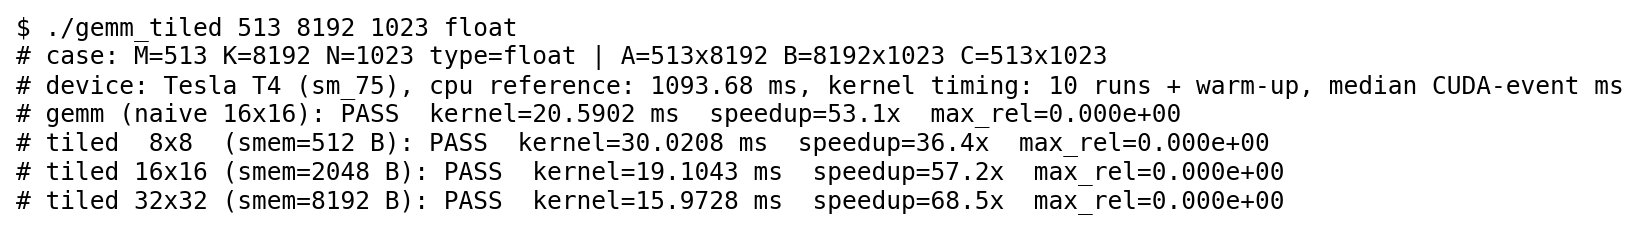
\includegraphics[width=\textwidth]{Q2/results/screenshots/q2_513x8192x1023_output.png}
\caption{Output for A \(513\times8192\) and B \(8192\times1023\). All output
elements pass full validation.}
\label{fig:q2-ragged}
\end{figure}

Here \(K=8192\) is divisible by all three tile sizes; \(M=513\) and \(N=1023\)
produce the partial boundary tiles. Zero-filled shared-memory padding gives the
same result as the CPU reference. The 32 tile is fastest at 15.9728\,ms, 1.29
times as fast as naive GEMM (20.5902\,ms). The 16 tile takes 19.1043\,ms, while
the 8 tile is slowest at 30.0208\,ms. The single-threaded CPU time is 1093.68\,ms.

\subsection*{4. Occupancy and shared memory}
\begin{table}[H]
\centering
\begin{tabular}{@{}lrrr@{}}
\toprule
Kernel & Dynamic shared memory & \multicolumn{2}{c}{Achieved occupancy (\%)} \\
\cmidrule(lr){3-4}
 & per block (B) & \(1024^3\) & \(513\times8192\times1023\) \\
\midrule
Naive \texttt{gemm} & 0 & 98.91 & 96.93 \\
Tiled \(8\times8\) & 512 & 98.69 & 97.56 \\
Tiled \(16\times16\) & 2,048 & 98.69 & 97.70 \\
Tiled \(32\times32\) & 8,192 & 99.96 & 99.99 \\
\bottomrule
\end{tabular}
\caption{Nsight Compute occupancy and shared-memory usage. Theoretical occupancy
is 100\% for every row.}
\label{tab:q2-occupancy}
\end{table}

None of these tests is limited by shared-memory capacity. The 32 tile has 1,024
threads and one resident block per SM, but that block contains all 32 warps and
achieved occupancy remains high. Low occupancy therefore cannot explain the 8
tile's time. Nsight Compute reports an 87.44\% L1 hit rate for naive GEMM in the
square case, compared with 25.68\%, 5.86\% and 0\% for the 8, 16 and 32 tiles.
Caching helps the naive kernel, which is why fewer load instructions do not
produce a proportional speed-up.

\subsection*{5. Increasing-size benchmark}
\begin{figure}[H]
\centering
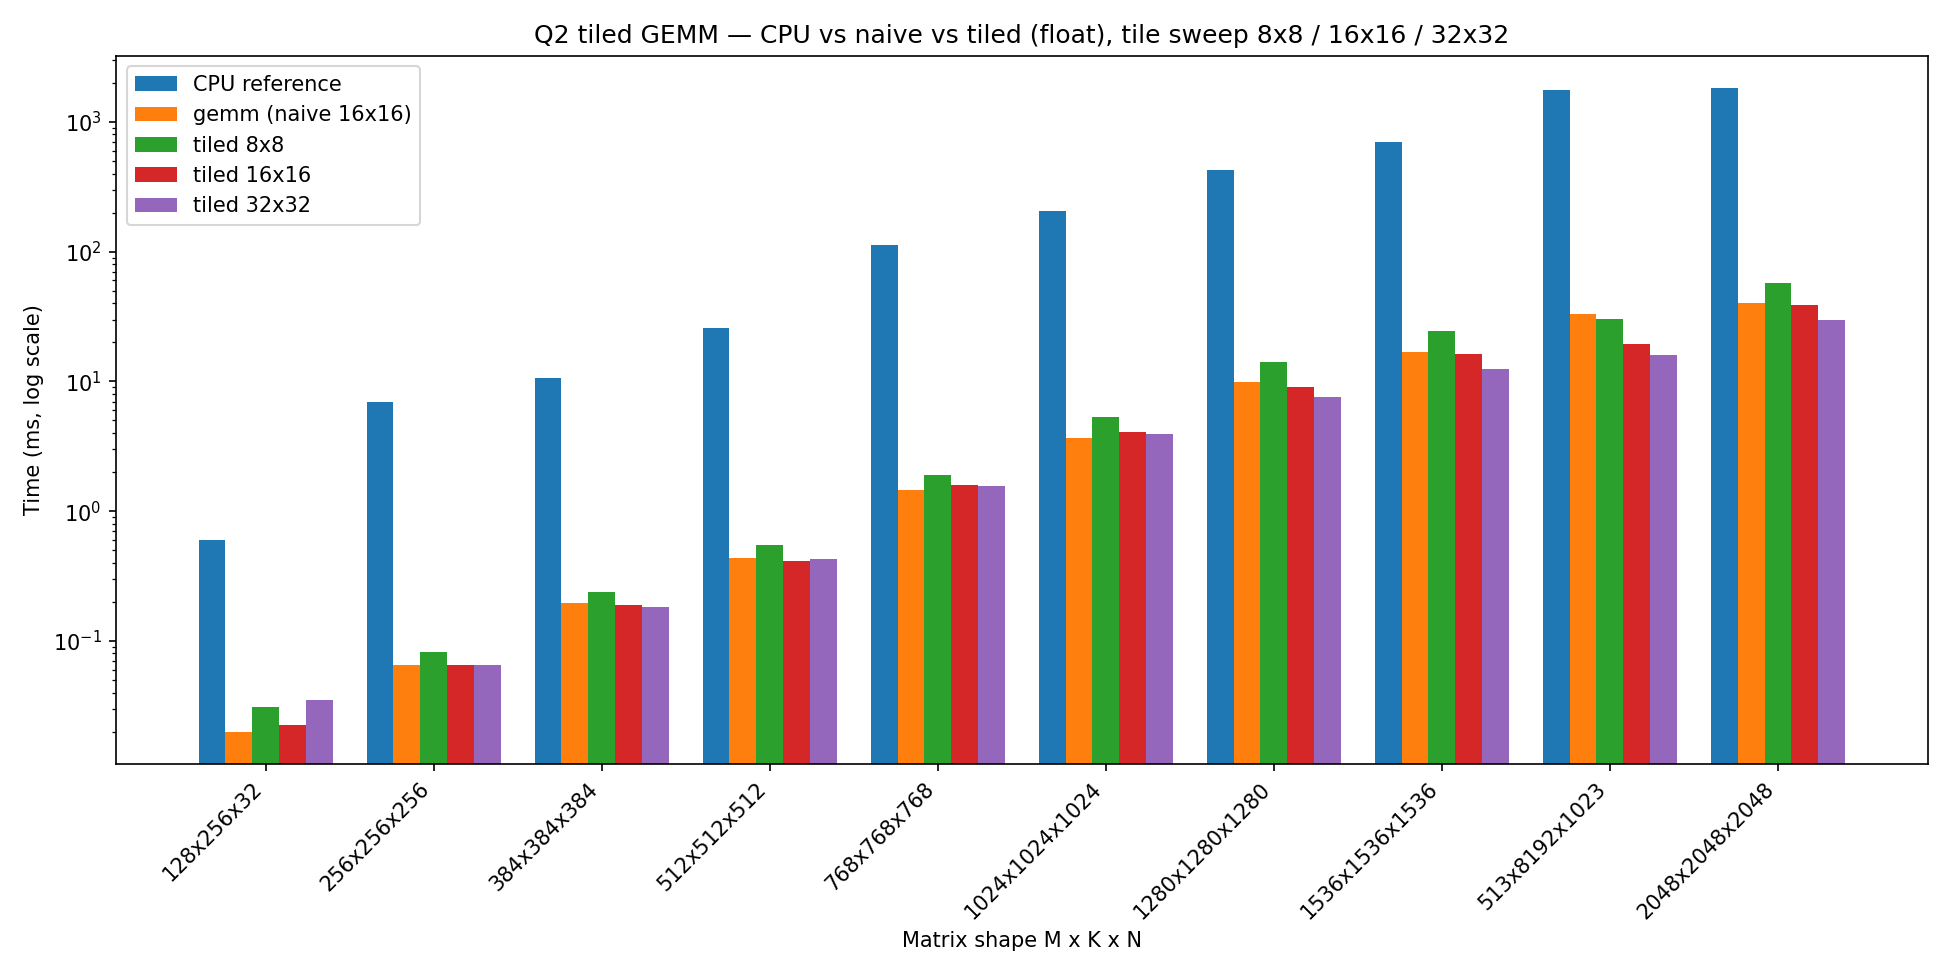
\includegraphics[width=\textwidth]{Q2/results/timing_float.png}
\caption{Ten-shape benchmark, ordered by total multiply-accumulate work. The
logarithmic axis compares the CPU, naive and three tiled kernels.}
\label{fig:q2-sweep}
\end{figure}

The naive kernel performs well on small and medium matrices. It is fastest for
\(128\times256\times32\), \(768^3\) and the sweep's \(1024^3\) run. Tiling adds
barriers, shared-memory stores and address calculations, while the naive kernel
benefits from its high cache hit rate. The 8 tile is never fastest. From
\(1280^3\) upward the 32 tile is fastest; at \(2048^3\) it takes 29.5035\,ms,
compared with 40.0891\,ms for naive and 1819.54\,ms on the CPU. Occupancy stays
high across these kernels. The unexpected behavior comes from the naive
kernel's cache use and the extra work performed by small tiles. Raw timings are
in \texttt{Q2/results/timing\_float.csv}, and the two \texttt{ncu\_*.txt} files
contain the profiling output.

% =====================================================================
\clearpage
\section*{Question 3 --- Accelerate Llama2 Inference}
\tocentry{Question 3 --- Accelerate Llama2 Inference}

\subsection*{Setup and implementation}
The runs used a Tesla T4 in Google Colab, with CUDA 13.0.88 and Nsight Systems 2025.3.1. For the CPU baseline, we compiled Karpathy's FP32 \texttt{run.c} with \texttt{gcc -O3} and ran \texttt{./run stories15M.bin}. For the comparison, all three versions used an empty prompt and the same flags, \texttt{-t 0 -s 42 -n 256}.

In the CUDA kernel, one thread computes the dot product of one weight row and the input vector. Each block has 128 threads. The naive version allocates three buffers and copies the input and weights to the GPU on each call. After the kernel it copies the result back and frees the buffers. The optimized version uploads the checkpoint once and finds each weight matrix by its offset. It uses the same kernel and reuses the input and output buffers.

\subsection*{Correctness and throughput}
The three runs generated identical text with the same flags. We also ran both CUDA versions with \texttt{CHECK\_MATMUL=1} for up to eight steps. This checked each output element against the CPU result \(y\), with a tolerance of \(10^{-5}+10^{-5}|y|\). Both passed. We used \texttt{--fmad=false} to keep multiplication and addition separate.

The CPU run with the counter made \textbf{9,546 matmul calls}. Each forward pass does seven matmuls per layer across six layers and one for the vocabulary output, giving \(7\times6+1=43\). The run stopped after 222 forward passes.

\begin{table}[H]
\centering
\begin{tabular}{@{}lrr@{}}
\toprule
\textbf{Run} & \textbf{Achieved tok/s} & \textbf{Relative to matched CPU} \\
\midrule
CPU, README command & 43.416167 & --- \\
CPU, matched workload & 45.926850 & \(1.00\times\) \\
Naive CUDA & 34.661230 & \(0.75\times\) \\
Optimized CUDA & 283.697047 & \(6.18\times\) \\
\bottomrule
\end{tabular}
\caption{Achieved tokens per second of the CPU and CUDA versions.}
\label{tab:q3-toks}
\end{table}

Figures~\ref{fig:q3-cpu}--\ref{fig:q3-opt} show the original notebook screenshots for the CPU README run and both CUDA runs.

\subsection*{Nsight Systems profiling}
We profiled both CUDA versions with the same input and flags. The profiles include the checkpoint upload during setup. The throughput values above come from separate runs, and their timer starts after the first forward pass.

\begin{table}[H]
\centering
\begin{tabular}{@{}lrr@{}}
\toprule
\textbf{Metric} & \textbf{Naive CUDA} & \textbf{Optimized CUDA} \\
\midrule
\multicolumn{3}{@{}l}{\textbf{CUDA Runtime API}} \\
\texttt{cudaMalloc} calls & 28,638 & 3 \\
\texttt{cudaMalloc} total (ms) & 1,182.28 & 184.77 \\
\texttt{cudaFree} calls & 28,638 & 3 \\
\texttt{cudaFree} total (ms) & 965.91 & 0.34 \\
\texttt{cudaMemcpy} calls & 28,638 & 19,093 \\
\texttt{cudaMemcpy} total (ms) & 4,600.70 & 725.04 \\
\addlinespace
\multicolumn{3}{@{}l}{\textbf{GPU memory copies and kernel}} \\
Host-to-device copies & 19,092 & 9,547 \\
Host-to-device data (MB) & 13,500.470 & 74.370 \\
Host-to-device total (ms) & 2,306.40 & 20.46 \\
Device-to-host copies & 9,546 & 9,546 \\
Device-to-host data (MB) & 44.272 & 44.272 \\
Device-to-host total (ms) & 18.87 & 15.42 \\
\texttt{matvec\_kernel} launches & 9,546 & 9,546 \\
\texttt{matvec\_kernel} total (ms) & 492.22 & 523.64 \\
\bottomrule
\end{tabular}
\caption{Nsight Systems summary of the naive and optimized CUDA versions.}
\label{tab:q3-nsys}
\end{table}

\textbf{Naive bottleneck.} The largest cost was copying the weights to the GPU on every call. Host-to-device copies took 2,306.40\,ms on the GPU, and the kernel took 492.22\,ms. In the CUDA API summary, \texttt{cudaMemcpy} accounted for 66.7\% of the recorded time. Allocation and release took another 31.1\%.

\textbf{After keeping weights on the GPU.} The optimized version uploaded the checkpoint once and copied 9,546 input vectors. That brought host-to-device traffic down to 74.370\,MB and copy time down to 20.46\,ms. It made three allocations at startup and freed the buffers at shutdown. The kernel count and the amount copied back to the CPU stayed the same. Total kernel time went from 492.22 to 523.64\,ms. The optimized version ran \textbf{\(8.18\times\) as fast as naive CUDA} and \textbf{\(6.18\times\) as fast as the matched CPU run}.

{\small The results are saved in \texttt{Q3/hw2\_Q3.ipynb}. The source ZIP contains the modified \texttt{run.c}, CUDA source and \texttt{Makefile}.
\href{https://github.com/karpathy/llama2.c/tree/350e04fe35433e6d2941dce5a1f53308f87058eb}{Upstream source}\enspace
\href{https://docs.nvidia.com/nsight-systems/AnalysisGuide/index.html}{Nsight Systems report guide}}

\subsection*{Benchmark screenshots}
\begin{figure}[H]
\centering
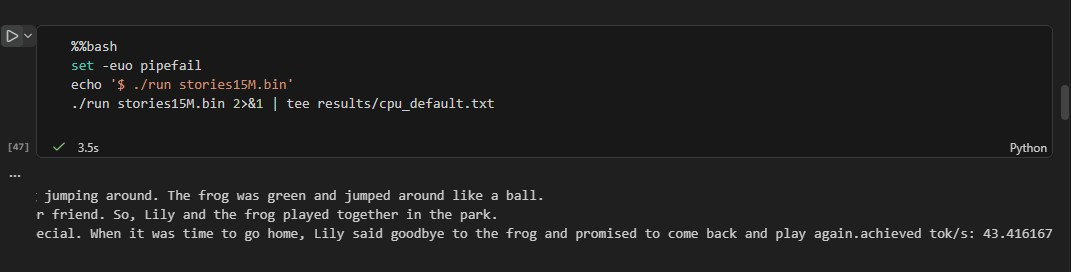
\includegraphics[width=\linewidth]{Q3/report_figures/47.jpg}
\caption{Original CPU backend, README command (execution 47).}
\label{fig:q3-cpu}
\end{figure}

\begin{figure}[H]
\centering
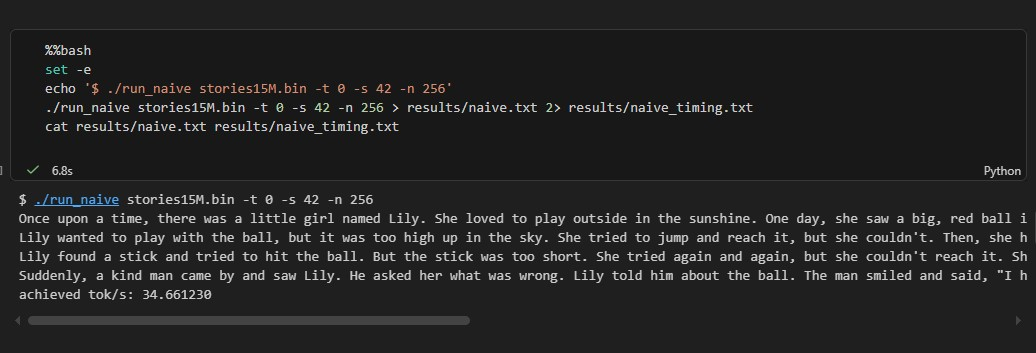
\includegraphics[width=\linewidth]{Q3/report_figures/49.jpg}
\caption{Naive CUDA backend, matched workload (execution 49).}
\label{fig:q3-naive}
\end{figure}

\begin{figure}[H]
\centering
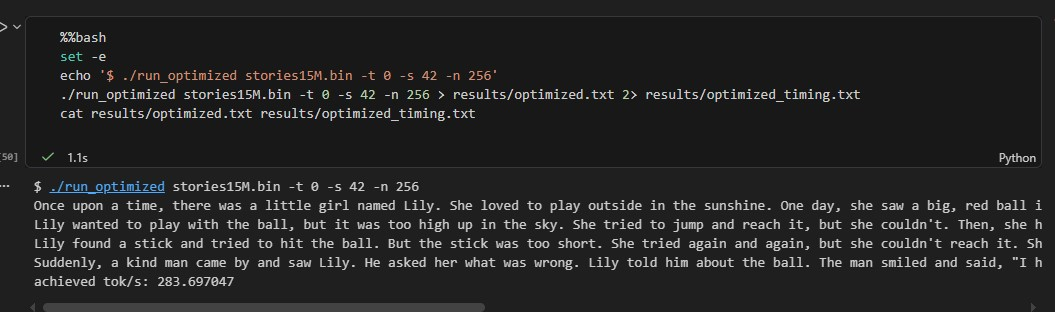
\includegraphics[width=\linewidth]{Q3/report_figures/50.jpg}
\caption{Optimized CUDA backend, matched workload (execution 50).}
\label{fig:q3-opt}
\end{figure}

% =====================================================================
% Optional bonus
\clearpage
\section*{Bonus --- A Particle Simulation Application}
\tocentry{Bonus --- A Particle Simulation Application}

\subsection*{1. Environment, build and execution}
The code is based on KTH-ScaLab/DD2360-HT25 at commit
\texttt{53e7ca59d190}. We used Google Colab with
a Tesla T4, driver 580.82.07 and CUDA 13.0.88. The revised Makefile builds
\texttt{miniPIC\_cpu.out}, \texttt{miniPIC\_gpu.out} and
\texttt{mover\_compare.out} with separate object directories. This prevents
CPU and GPU objects from contaminating each other. \texttt{ARCH=sm\_75} selects
the T4 architecture; the CPU target needs only \texttt{g++}.

We ran the unmodified \texttt{GEM\_2D.inp} for all ten cycles:
\begin{verbatim}
make -j2 cpu
make -j2 gpu compare ARCH=sm_75
./bin/mover_compare.out inputfiles/GEM_2D.inp
cd .. && ./run_compare.sh
\end{verbatim}
The last command runs both complete simulations and compares their VTK output.

\subsection*{2. GPU mover design}
The original CPU \texttt{mover\_PC()} is retained. The new
\texttt{mover\_PC\_gpu()} allocates device buffers on each call, uploads six
particle arrays, six field arrays and three grid-coordinate arrays, launches
one thread per particle, and copies the six updated particle arrays back. Each
thread executes its particle's subcycles and predictor--corrector iterations
sequentially. It performs the same trilinear interpolation, velocity solve and
periodic/reflecting boundary updates as the CPU version.

The upstream contiguous flat arrays are copied directly. Device addressing follows
\(n_{yn}n_{zn}i_x+n_{zn}i_y+i_z\), so no host pointer chain is copied. Grid
constants are passed by value. CUDA calls and launch errors are
checked, and RAII wrappers release buffers and events on error paths. CUDA
events measure kernel time separately from end-to-end mover time.

\subsection*{3. CPU/GPU correctness}
The standalone checker starts from one \texttt{initGEM} state and compares every
\(x,y,z,u,v,w\) value for all four species. This covers 16,384,000 particles
and 98,304,000 values. All values passed
\(|g-c|\leq10^{-4}+10^{-3}|c|\). The worst absolute error was
\(3.8147\times10^{-6}\). A worst relative error of 1 occurs only for a near-zero
velocity whose absolute error is \(5.96046\times10^{-8}\).

\begin{figure}[H]
\centering
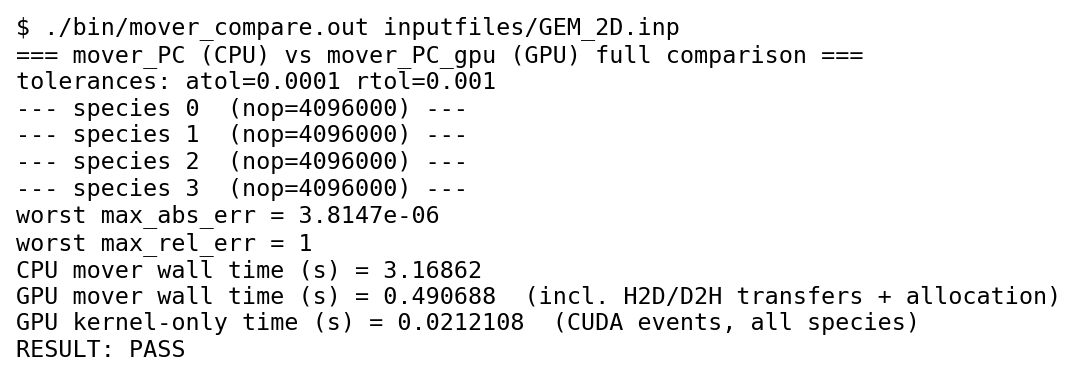
\includegraphics[width=0.95\textwidth]{Bonus/results/screenshots/bonus_mover_compare.png}
\caption{Full CPU/GPU mover comparison on the Tesla T4.}
\label{fig:bonus-mover}
\end{figure}

Both complete simulations also finished ten cycles. E and B at cycle 10 were
byte-identical. Every value in the three density files passed the numerical
comparison; the maximum absolute errors were \(10^{-7}\) for electron density,
\(10^{-13}\) for ion density and \(3\times10^{-8}\) for net density. Thus all
five VTK files passed. The checker also rejects NaN and infinity rather than
allowing them to compare as equal. Raw logs and numerical comparisons are in
\texttt{Bonus/results/}.

\subsection*{4. Execution time}
\begin{table}[H]
\centering
\begin{tabular}{@{}lrr@{}}
\toprule
Complete GEM\_2D run & CPU (s) & GPU (s) \\
\midrule
Total simulation & 61.9111 & 30.9489 \\
Mover per cycle, end-to-end & 3.35445 & 0.249392 \\
Mover kernel per cycle & --- & 0.0237013 \\
Interpolation per cycle & 2.47386 & 2.47776 \\
\bottomrule
\end{tabular}
\caption{CPU/GPU timing for the complete ten-cycle simulation.}
\label{tab:bonus-timing}
\end{table}

The end-to-end mover speed-up is \textbf{13.45x}, including allocation and all
transfers. Allocation, transfers and launch overhead account for 0.22569\,s,
90.5\% of the GPU mover time. The whole simulation is \textbf{2.00x} as fast;
its remaining hotspot is CPU interpolation, which takes about 2.48\,s per cycle
in both runs.

\end{document}
